
% ===============================================

\documentclass[a4paper]{article}
\usepackage[margin=1in]{geometry}
\usepackage{textpos}
\usepackage{enumerate}
\usepackage{amsmath,amsthm,amssymb}
\usepackage[english]{babel}
\usepackage[utf8]{inputenc}
\usepackage{alltt}
\usepackage[]{algorithm2e}
\usepackage{mathtools}
\usepackage{graphicx}

\DeclarePairedDelimiter\ceil{\lceil}{\rceil}
\DeclarePairedDelimiter\floor{\lfloor}{\rfloor}
\begin{document}

% ------------------------------------------ %
%                 START HERE                 %
% ------------------------------------------ %

\title{Variational Canonical Correlation Analysis (VCCA)} % Replace "1" with the appropriate number
\author{Yang Chen} % Replace "Author's Name" with your name
\maketitle
\section{Multi-View Learning task}
In the multi-view representation learning setting, we have multiple views (types of measurements) of the same under- lying signal, and the goal is to learn useful features of each view using complementary information contained in both views. The learned features should uncover the common sources of variation in the views, which can be helpful for exploratory analysis or for downstream tasks.
\section{VCCA}
VCCA models the {\bf joint distribution of two views} with a latent variable model capturing both the shared and private information, where the distributions are parameterized by deep neural networks. VCCA optimizes a {\bf variational lower bound} of the likelihood and allows for straightforward training using small minibatches of training samples.
\section{Latent Variable}
\subsection{}

The probabilistic latent variable model interpretation of linear CCA is shown hare:

\begin{center}
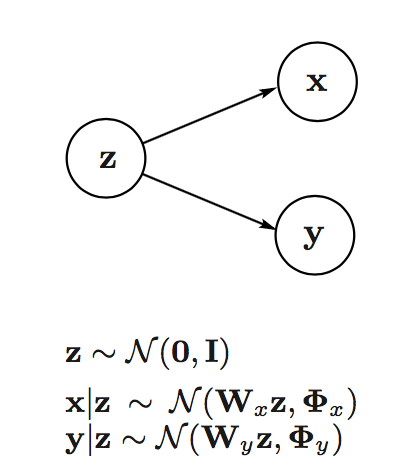
\includegraphics[width=4cm, height=5cm]{lat.png}
\end{center}

Assuming that x and y are linear functions of some random variable z in $R^{d_z}$, where $d_z <= min(d_x,d_y)$. The prior distribution p(z) and conditional distributions $p(x|z)$ and $p(y|z)$ are Gaussian. Jordan showed that $E(z|x)$ lives in the same space as the linear CCA projection for x.

The VCCA model extends the latent variable interpretation of linear CCA to nonlinear observation models parameterized by DNN.
\begin{center}
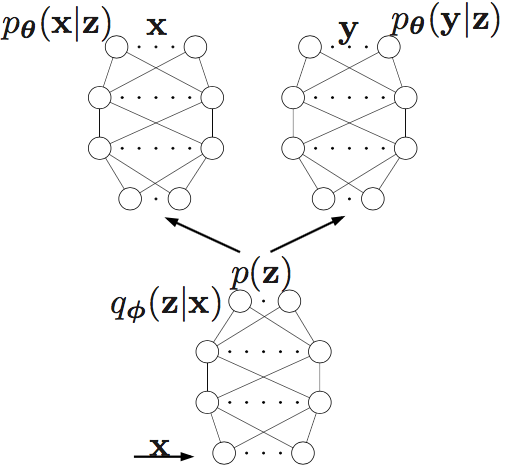
\includegraphics[width=5cm, height=5cm]{vcca.png}

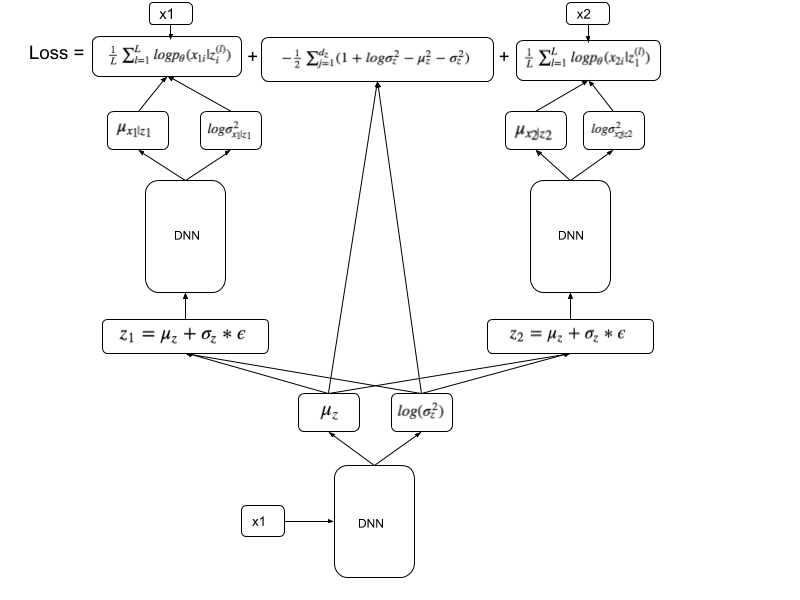
\includegraphics[width=15cm, height=12cm]{vcca_nn.png}
\end{center}
The probabilistic latent variable model of CCA defines the following joint distribution over the random variables (x,y):
    
$p(x,y,z) = p(z)p(x|z)p(y|z)$

$p(x,y)=\int p(x,y,z)dz$

Assumption: x and y are conditionally independent on z.

However, $p_\theta(x,y)$ does not have a closed form, and $p_\theta(z|x)$ is intractable. (Reason: This integral requires exponential time to compute as it needs to be evaluated over all configurations of {\bf latent variables}. So we need to approximate this posterior distribution.)

\section{Objective}
\subsection{Lower Bound}

$logp_\theta(x,y) >= L(x,y;\theta,\Phi) := - D_{KL}(q_\Phi(z|x)||p(z)) + E{q_\Phi(z|x)}[logp_\theta(x|z)+logp_\theta(y|z)]$
\subsection{Derivation of the lower bound}
\begin{align*}
log_{p\theta}(x,y)\\
&= log_{p\theta}(x,y) \int q_\Phi(z|x)dz\\
&= \int log_{p\theta}(x,y) q_\Phi(z|x)dz\\
&= \int q_\Phi(z|x) (log(p(x,y,z)/p(z|x,y)))dz\\
&= \int q_\Phi(z|x) (log(p(x,y,z)/q(z|x)* q(z|x)/p(z|x,y)) dz\\
&= \int q_\Phi(z|x) log\frac{p(x,y,z)}{q(z|x)}dz + \int q_\Phi(z|x) log\frac{q(z|x)}{p(z|x,y)}dz\\
&= E_{q\Phi(z|x)}[log\frac{p_\theta(x,y,z)}{q_\Phi(z|x)}]+ D_{KL}(q_\Phi(z|x)||p_\theta(z|x,y))\\
&>= E_{q\Phi(z|x)}[log\frac{p_\theta(x,y,z)}{q_\Phi(z|x)}] \to (\text{KL is nonnegative})\\
&= L(z,y;\theta,\Phi)
\end{align*}

So 

\begin{align*}
L(x,y;\theta,\Phi)\\
&= \int q_\Phi(z|x)[log \frac{p(z)p(x|z)p(y|z)}{q(z|x)}]dz\\
&= \int q_\Phi(z|x)[log \frac{p(z)}{q(z|x)} + logp(z|x) logp(y|z)]dz\\
&= - D_{KL}(q_\Phi(z|x)||p(z)) + E_{q(z|x)}[log p(x|z) + log p(y|z)]
\end{align*}

\subsection{Compute E part}

$E_{q\Phi(z_i|x_i)}[logp_\theta(x_i|z_i) + logp_\theta(y_i|z_i)]=\frac{1}{L}\sum_{l=1}^L logp_\theta(x_i|z_i^{(l)})+logp_\theta(y_i|z_i^{(l)})$

\subsubsection{Code}
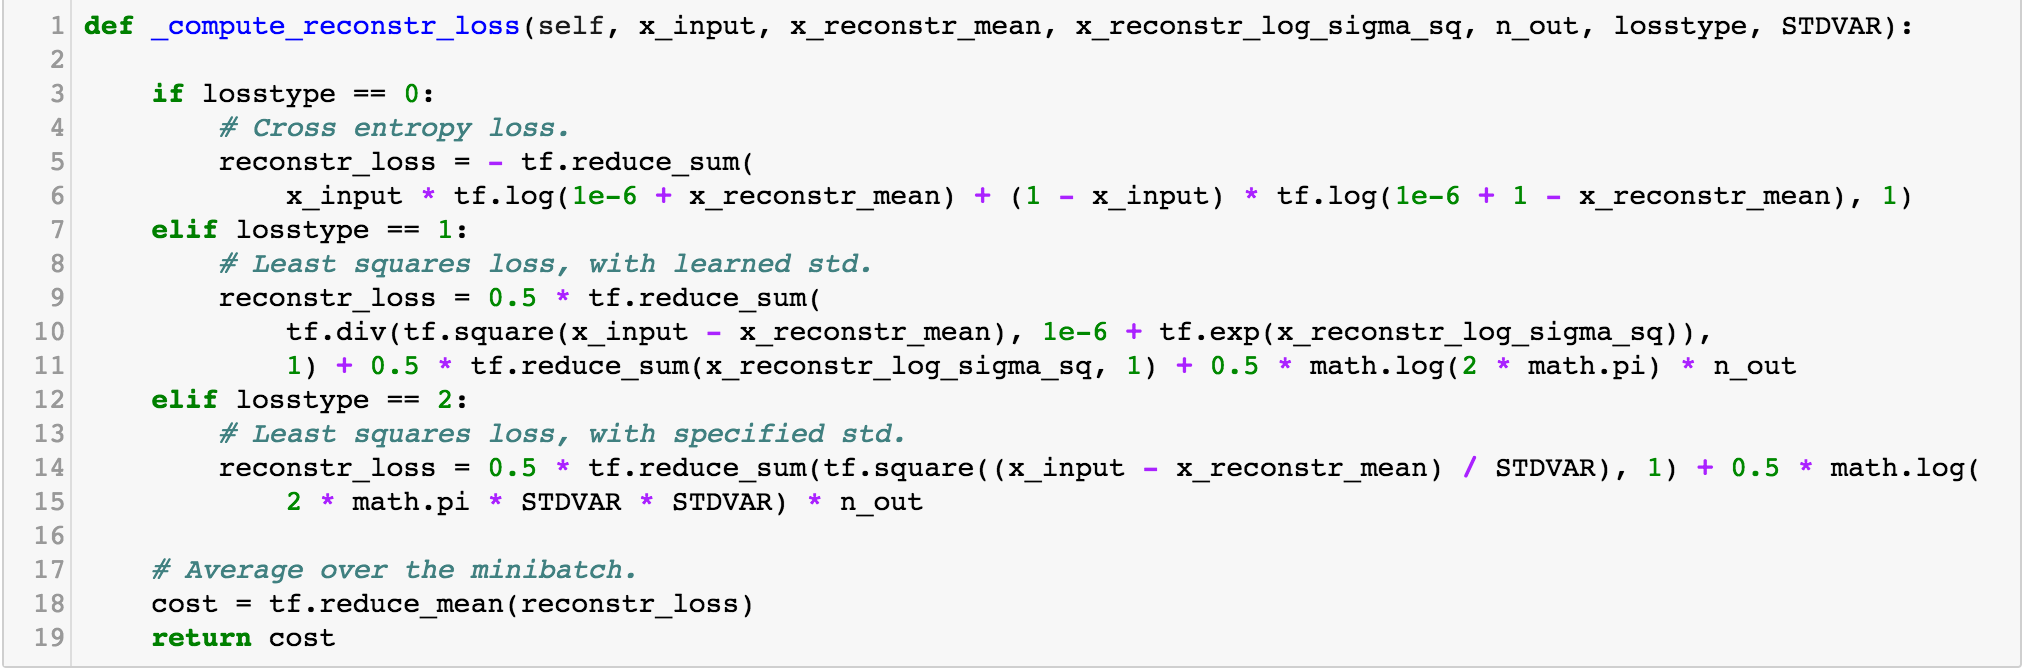
\includegraphics[width=17cm, height=6cm]{loss_code.png}

\subsection{Compute KL divergence}

$D_{KL}(q_\Phi(z_i|x_i)||p(z_i)) = -\frac{1}{2}\sum_{j=1}^{d_z}(1+log\sigma_{ij}^2 - \sigma_{ij}^2 - \mu_{ij}^2)$


\subsubsection{Derivation of KL divergence}
Assumption random variable x1,x2 is Gaussian distribution. $x1\to N_1(\mu_1,\sigma_1^2), x2\to N_2(\mu_2,\sigma_2^2)$. 

$N(\mu,\sigma^2) = \frac{1}{\sqrt{2\pi\sigma^2}}e^{\frac{(x-\mu)^2}{2\sigma^2}}$

\begin{align*}
&\int p_1(x)log\frac{p_1(x)}{p_2(x)} dx\\
&= \int p_1(x) (logp_1(x) - logp_2(x))dx\\
&= \int p_1(x) (log \frac{1}{\sqrt{2\pi\sigma_1^2}}e^{\frac{(x-\mu_1)^2}{2\sigma_1^2}} -log \frac{1}{\sqrt{2\pi\sigma_2^2}}e^{\frac{(x-\mu_2)^2}{2\sigma_2^2}})dx\\
&= \int p_1(x) (-1/2 log2\pi - log\sigma_1 - \frac{(x-\mu_1)^2}{2\sigma_1^2} + 1/2 log2\pi + log \sigma_2 + \frac{(x-\mu_2)^2}{2\sigma_2^2})dx\\
&= \int p_1(x)(log\frac{\sigma_1}{\sigma_2} + [\frac{(x-\mu_1)^2}{2\sigma_1^2} - \frac{(x-\mu_2)^2}{2\sigma_2^2}]) dx\\
&= \int (log\frac{\sigma_2}{\sigma_1}p_1(x)dx + \int \frac{(x-\mu_1)^2}{2\sigma_1^2} p_1(x)dx - \int \frac{(x-\mu_2)^2}{2\sigma_2^2} p_1(x) dx\\
&= log\frac{\sigma_1}{\sigma_2} + \frac{1}{2\sigma_2^2}\int (x-\mu_2)^2p_1(x)dx - \frac{1}{2\sigma_1^2}\int (x-\mu_1)^2 p_1(x)dx\\
&= log\frac{\sigma_1}{\sigma_2} + \frac{1}{2\sigma_2^2}\int (x-\mu_2)^2p_1(x)dx - \frac{1}{2} \to (\int (x-\mu_1)^2 p_1(x)dx=\sigma_1^2)\\
&= log\frac{\sigma_1}{\sigma_2} + \frac{1}{2\sigma_2^2}\int (x-\mu_1+\mu_1-\mu_2)^2p_1(x)dx - \frac{1}{2}\\
&= log\frac{\sigma_1}{\sigma_2} + \frac{1}{2\sigma_2^2}[\int (x-\mu_1)^2p_1(x)dx + \int (\mu_1-\mu_2)^2p_1(x)dx + 2\int(x-\mu_1)(\mu_1-\mu_2)p_1(x)dx] - \frac{1}{2}\\
&=log\frac{\sigma_1}{\sigma_2} + \frac{1}{2\sigma_2^2}[\int (x-\mu_1)^2p_1(x)dx +(\mu_1-\mu_2)^2] - \frac{1}{2}\\
&\to (2\int(x-\mu_1)(\mu_1-\mu_2)p_1(x)dx = (\mu_1-\mu_2)\int (x-\mu_1)p_1(x)dx \\
&= (\mu_1-\mu_2)[\int xp_1(x)dx - \int \mu_1p_1(x)dx] = (\mu_1-mu_2)[\mu_1-\mu_1]=0\\
&= log\frac{\sigma_2}{\sigma_1}+\frac{\sigma_1^2+(\mu_1-\mu_2)^2}{2\sigma_2^2} - \frac{1}{2})\\
&\text{Let }\mu_2 = 0, \sigma_2^2 = 1\\
&= -log \sigma_1 + \frac{\sigma_1^2+\mu_1^2}{2}-\frac{1}{2}\\
&= -\frac{1}{2}(1 + 2log \sigma_1 - \sigma_1^2-\mu_1^2)\\
&= -\frac{1}{2}(1 + log \sigma_1^2 - \sigma_1^2-\mu_1^2)
\end{align*}

\subsubsection{Code}

\includegraphics[width=17cm, height=0.8cm]{kl_code.png}
\section{Reparameterization trick}

Intuitively, in its original form, VAEs sample from a random node z which is approximated by the parametric model $q(z | \Phi,x)$ of the true posterior. Backprop cannot flow through a random node.

Introducing a new parameter $\epsilon$ allows us to reparameterize z in a way that allows backprop to flow through the deterministic nodes.
\begin{center}
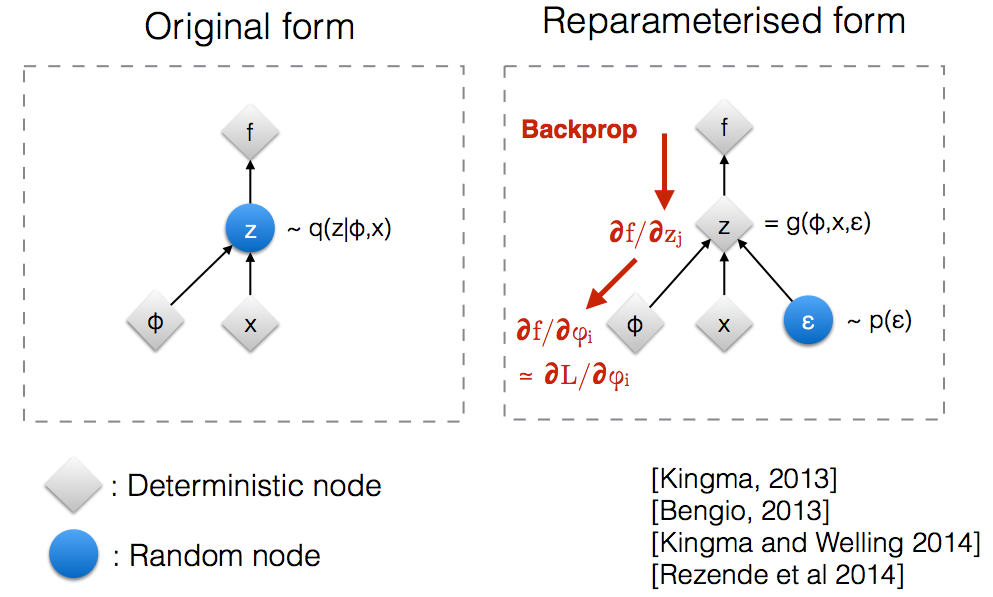
\includegraphics[width=10cm, height=6cm]{repara.png}
\end{center}
\subsection{Code}
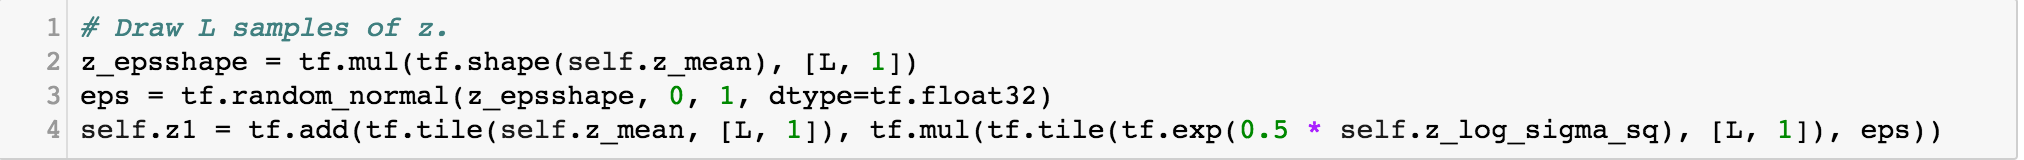
\includegraphics[width=17cm, height=1.5cm]{repa_code.png}
\section{Deep Neural Network}

We consider non-linear observation models $p_\theta(x|z;\theta_x), p_\theta(y|z;\theta_y)$, parameterized by $\theta_x$ and $\theta_y$, which can be the collections of weights of DNNs. We also approximate $p_\theta(z|x)$ with the conditional density $q_\Phi(z|x;\Phi_z)$, where $\Phi_z$ is the collection of parameters of another DNN.

\subsection{Code}

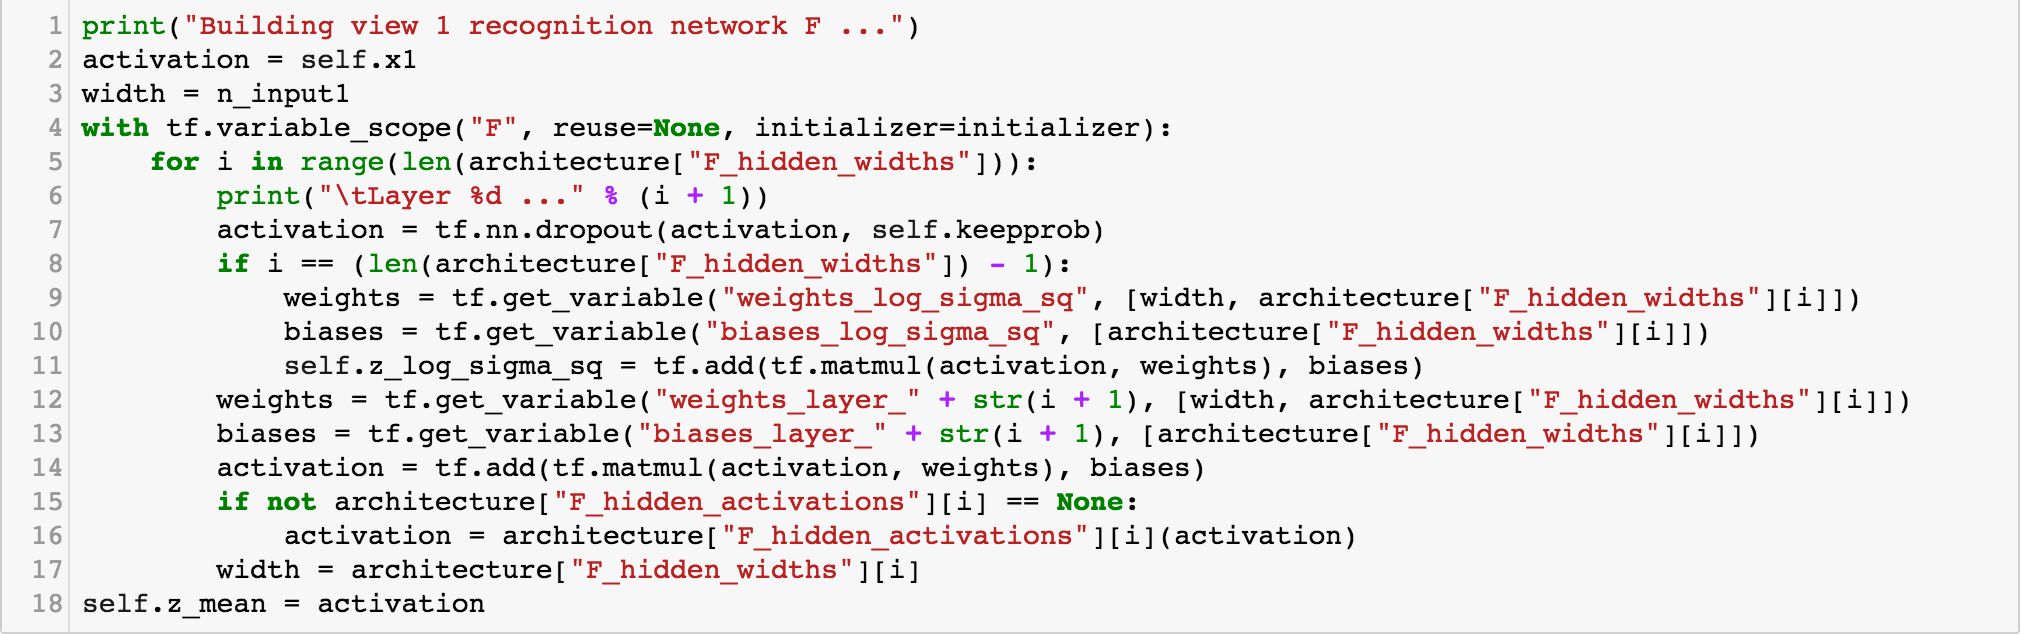
\includegraphics[width=17cm, height=6cm]{dnn_code.png}

\section{Private information}
There might be large variations in the input space that can not be explained by the common variables. It may then be beneficial to explicitly model the private variables within each view.
\begin{center}
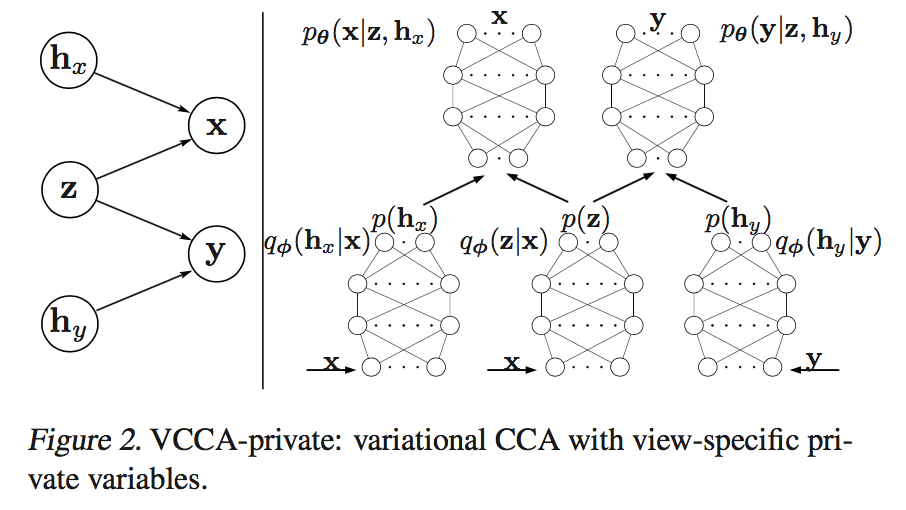
\includegraphics[width=10cm, height=6cm]{vcca-p.png}
\end{center}
% -----------------------------------------------
% Ignore everything that appears below this.
% -----------------------------------------------
\end{document}
